% Example results
\subsection{Simulation Outline}
The simulation results are images that were created using a specific interferometer layout and a specific sky model. The sky model that was used for the following results was a sky model with 4 points, each of which having a different brightness, or flux. The sky model can be seen below. 
\begin{center}
    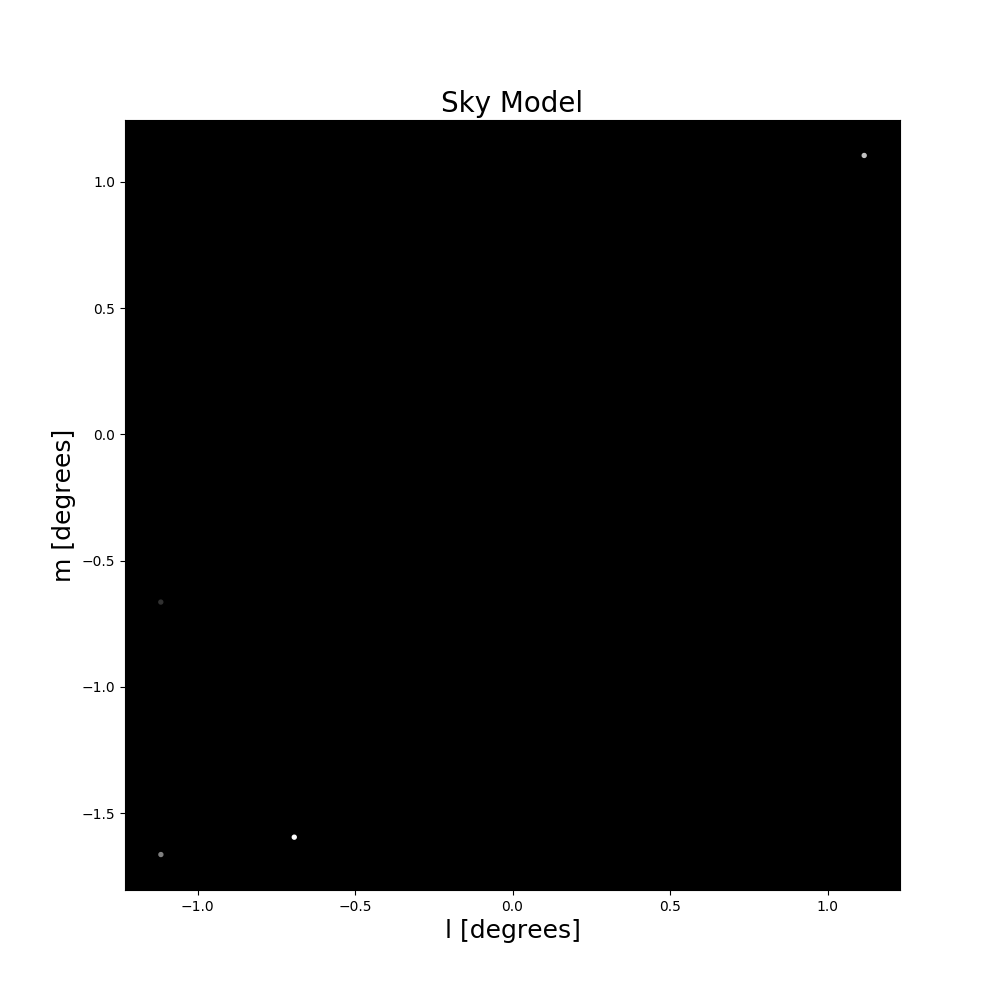
\includegraphics[scale=0.4]{images/4_POINT.png}
\end{center}
The sky model has a distinctive shape to it, the results from each interferomter should have this shape with a point spread function creating some noise around every point source. \\
Before the results are shown, the point spread functions for KAT 7, HERA 19 and TART will be displayed. These are the interferomters that were used to display the results, the TART interferometer here is a antenna layout that was created from TART's actual layout, it is simple treated here as a tracking array, while in reality it is in fact, not a tracking array.
\begin{figure}[htp]
  \centering
  \begin{subfigure}[b]{0.3\textwidth}
    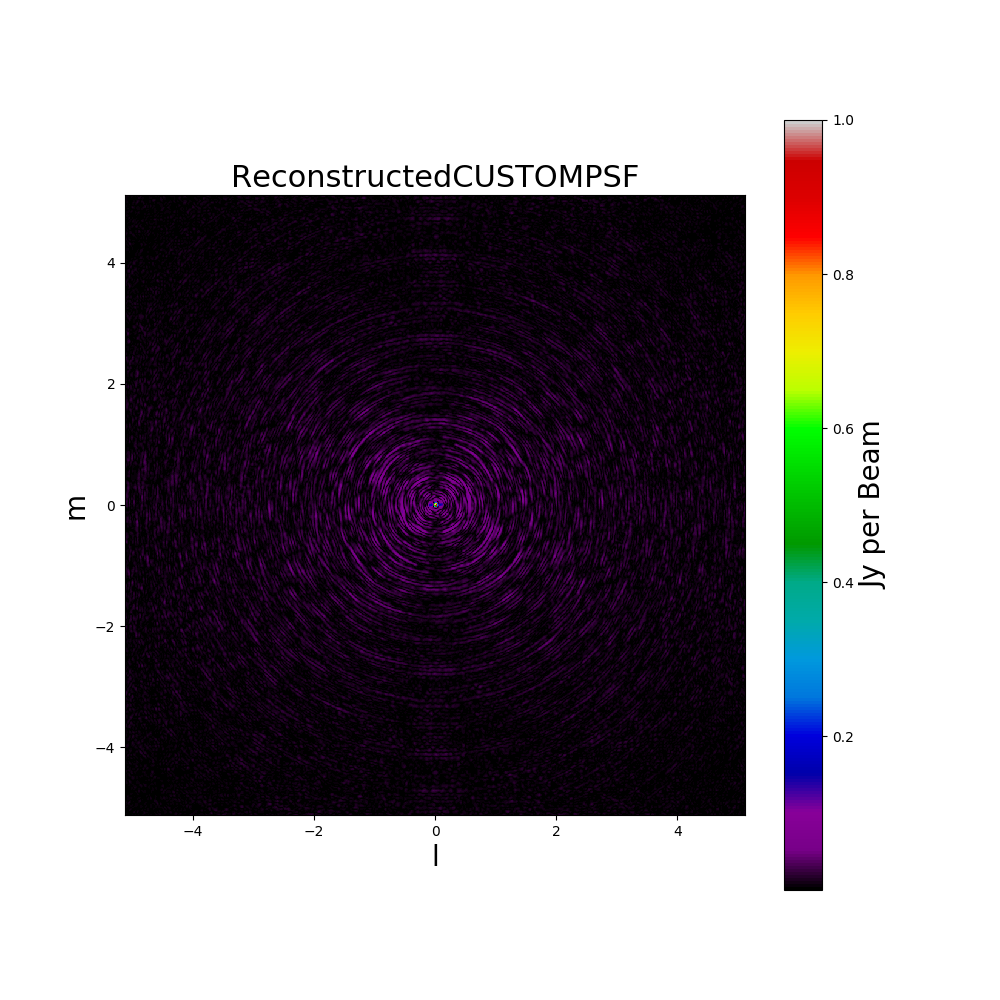
\includegraphics[width=\textwidth]{images/KAT_7_PSF.png}
    \caption{KAT 7 PSF}
    \label{fig:1}
  \end{subfigure}
  %
  \begin{subfigure}[b]{0.3\textwidth}
    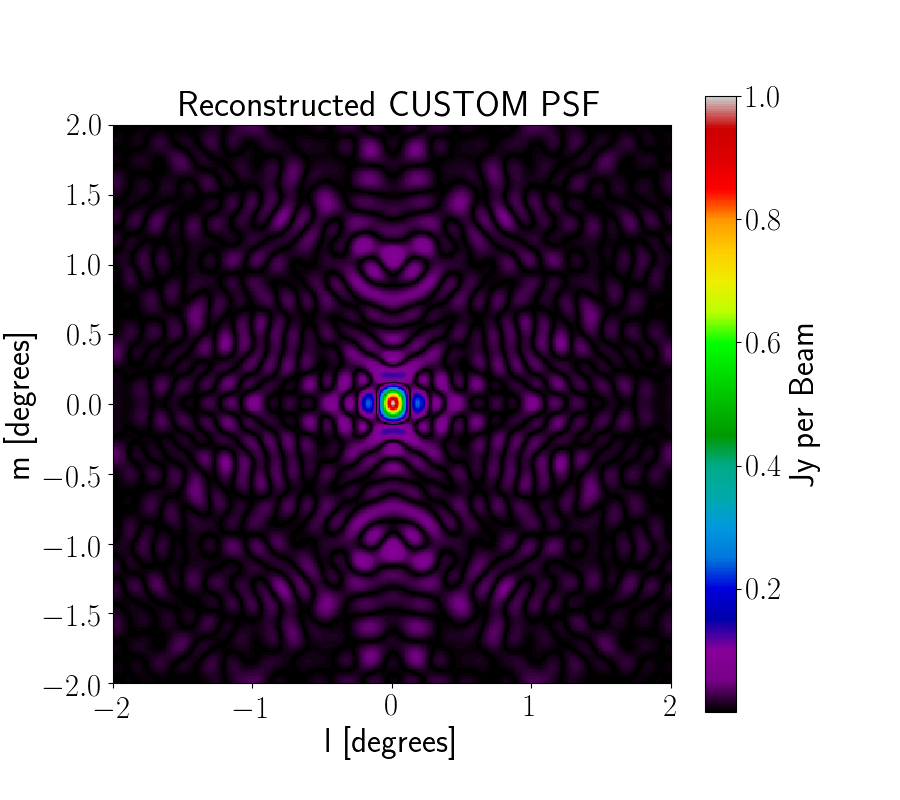
\includegraphics[width=\textwidth]{images/HERA_19_PSF.png}
    \caption{HERA 19 PSF}
    \label{fig:2}
  \end{subfigure}
  %
  \begin{subfigure}[b]{0.3\textwidth}
    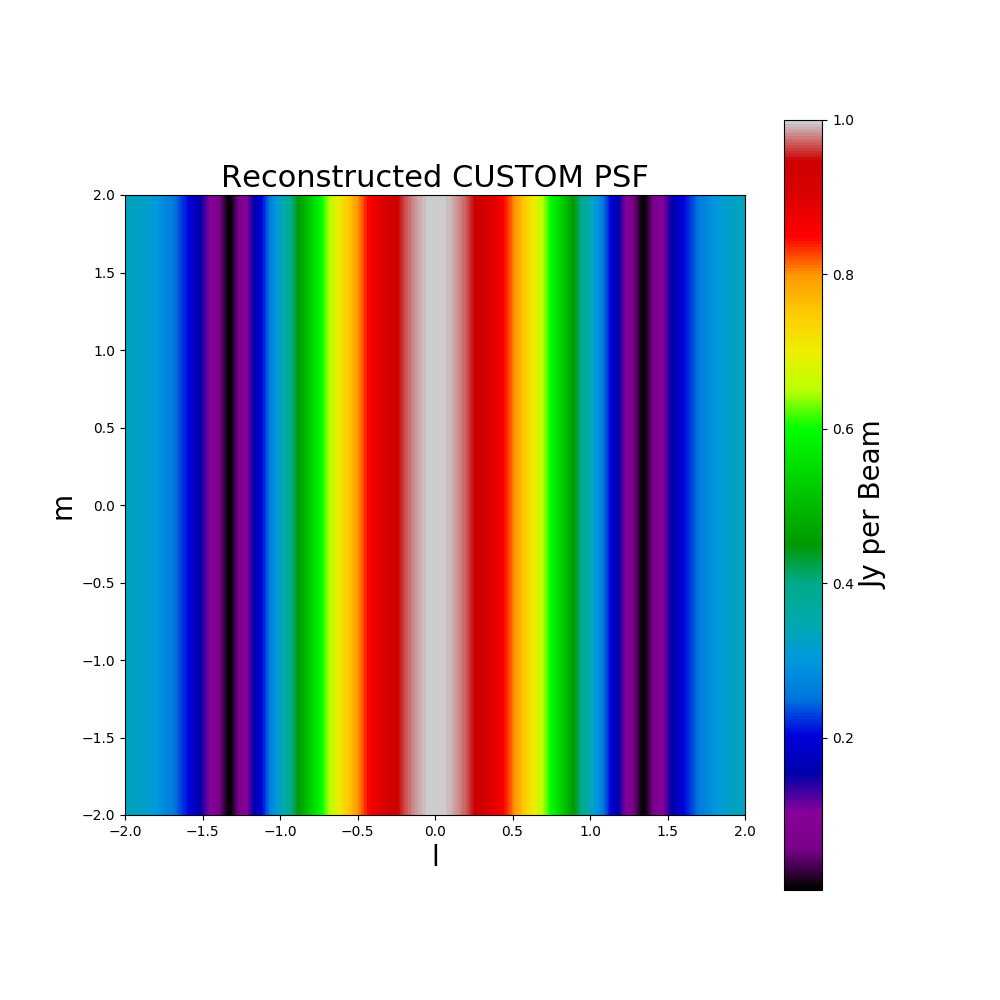
\includegraphics[width=\textwidth]{images/TART_PSF.png}
    \caption{TART PSF}
    \label{fig:2}
  \end{subfigure}
\end{figure}
\subsection{Simulation Results}
Below is a reconstruction from KAT 7 for this sky model using a cell size of $0.01^\circ$ and a resolution of $10^\circ$. 
\begin{center}
    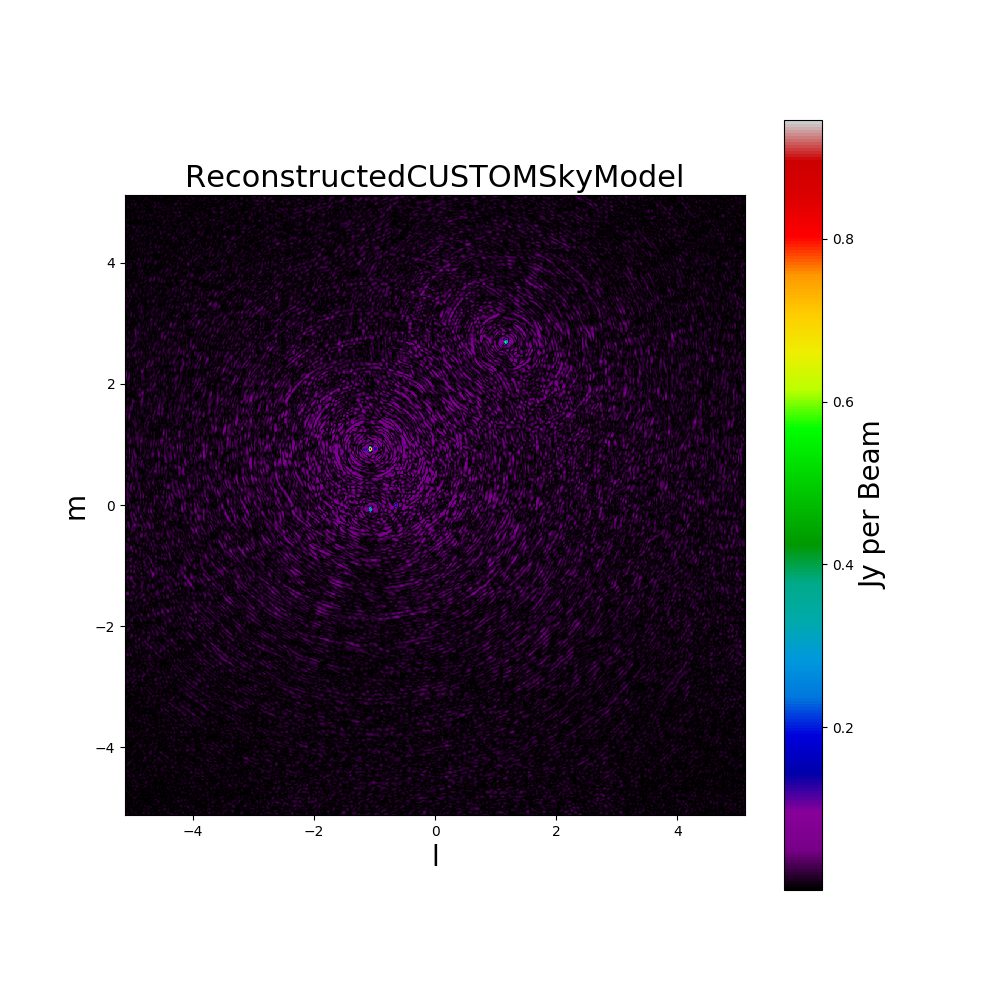
\includegraphics[scale=0.4]{images/RECON_KAT_7_4_POINT.png}
\end{center}
In this image it can be seen that the brighter sources are easily visible, but the one source that was not as bright is not nearly as visible.  The shape is correct and it can clearly be seen that the point spread function has introduced noise to the image and that it matches the point spread function that was introduced earlier in this section.\\
Below is a reconstruction from KAT 7 for this sky model using a cell size of $0.01^\circ$ and a resolution of $3^\circ$. 
\begin{center}
    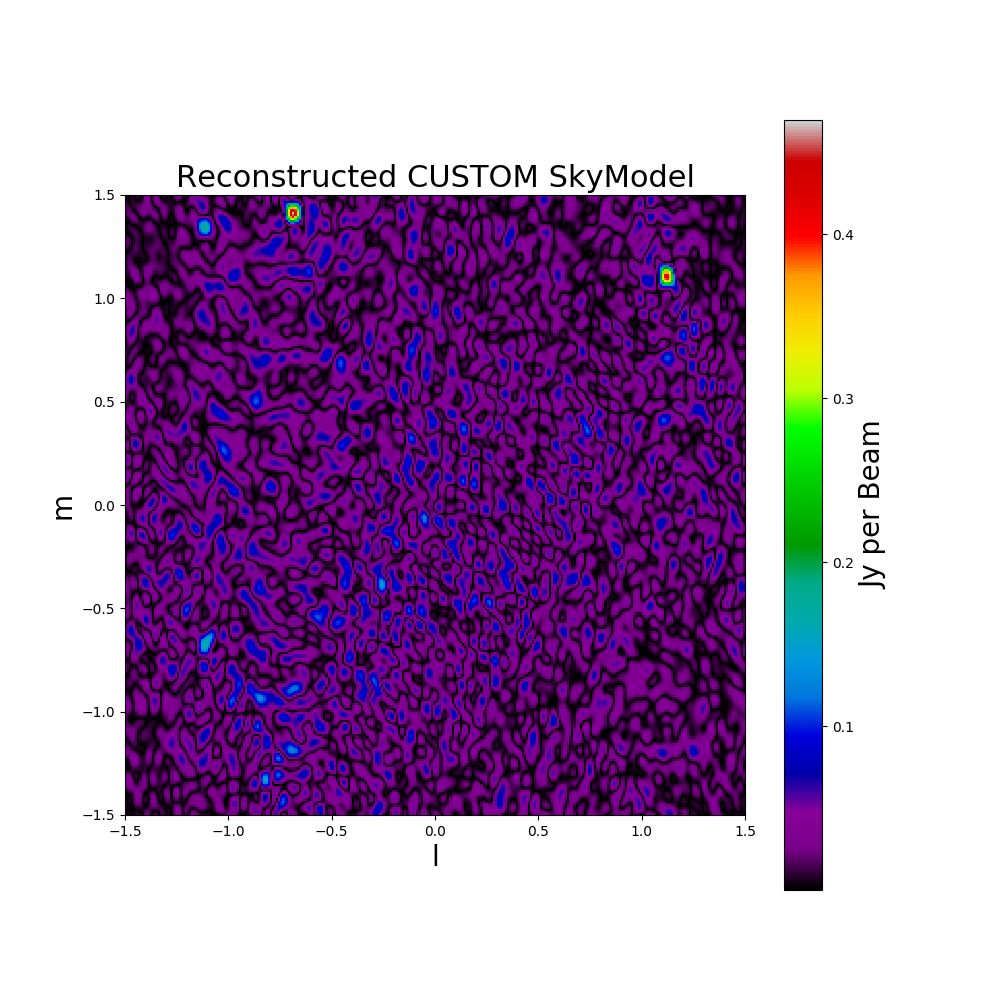
\includegraphics[scale=0.4]{images/RECON_KAT_7_4_POINT_ALIASING.png}
\end{center}
In this image the source at the top appears to be in the wrong location, this is due to aliasing as the resolution was not correctly selected. It is important to remember to follow the Nyquist Theorem that is outlined in section 2.4.1.

Below is a reconstruction from HERA 19 for the sky model using a cell size of $0.01^\circ$ and a resolution of $10^\circ$. 
\begin{center}
    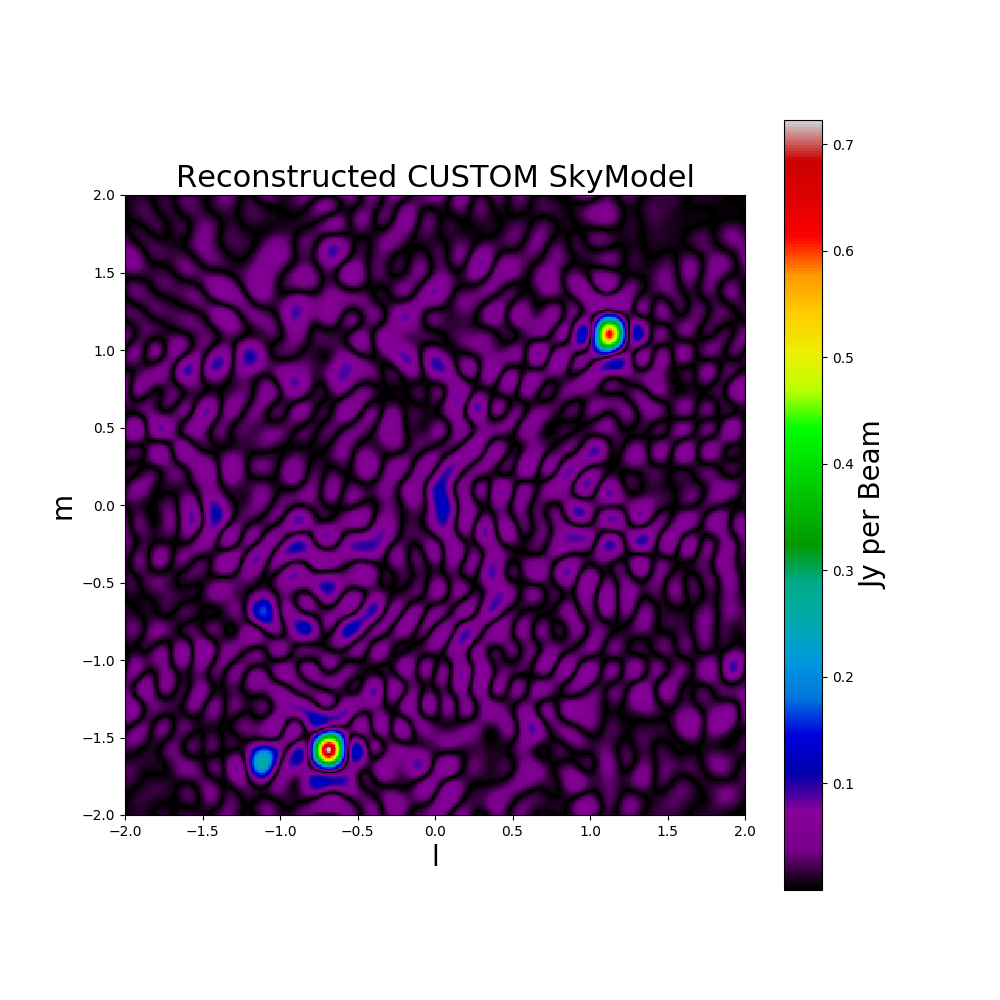
\includegraphics[scale=0.4]{images/RECON_HERA_19_4_POINT.png}
\end{center}
As with the KAT 7 image, the bright sources are easily visible while the one less bright source is hard to identify. The point spread function has introduced noise to the image around the sources and it is clear that it is the same point spread function that was shown earlier in this section.

Below is a reconstruction from TART for the sky model using a cell size of $0.01^\circ$ and a resolution of $10^\circ$. 
\begin{center}
    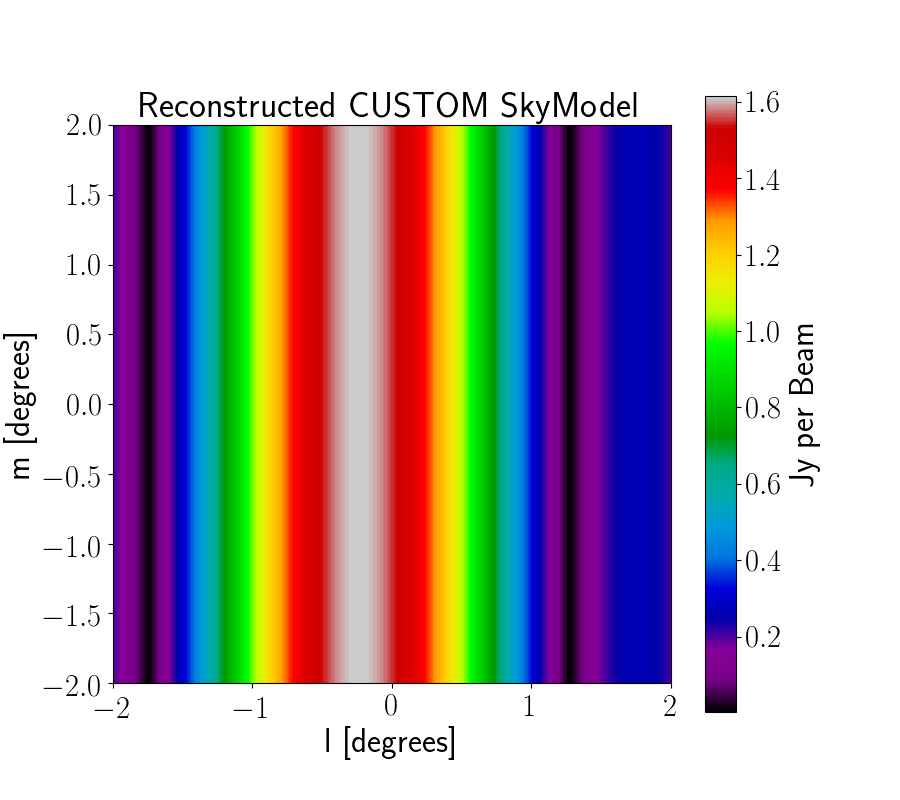
\includegraphics[scale=0.4]{images/RECON_TART_4_POINT.png}
\end{center}
It is instantly clear that the points are not at all visible in this reconstruction, this is because TART is not nearly as powerful as KAT 7 or HERA 19, it is also due to the very small hour angle that was given to TART for this simulation.

\subsection{TART Images}

\subsection{Conclusion}
The pipeline works correctly if the correct resolution is chosen for the images and if the user selects the correct cell size.\\
The images obtained from TART do not show much detail as TART is not a very powerful interferometer. As such, the results that are obtained from it will never match what is being produced by larger projects. So images will never show high levels of detail. TART is also a whole sky interferometer, this also means that the images are less detailed as they don't focus on a small area of the sky which would allow for higher details.
% It is however a perfect tool to teach students how radio interferometry works and if this pipeline was turned into a teaching tool it could explain the subject matter while having a real interferometer to show results with.

% Show simulation
%  Image from TART as final result